\chapter{Forces et champs}

\textit{La notion de champ est l’un des concepts les plus féconds de la physique. Elle permet de décrire l’action à distance exercée par une masse (champ gravitationnel), par une charge électrique (champ électrostatique) ou par un aimant (champ magnétique). Ce chapitre introduit ces trois champs fondamentaux, leurs sources, leurs représentations par des lignes de champ et leur superposition.}

% ===================================================================
\section{Notion de champ}

\begin{definition}[Champ]
Un \textbf{champ} est une grandeur physique définie en tout point de l’espace. On distingue :
\begin{itemize}
\item les \textbf{champs scalaires} (température, pression, potentiel) : une seule valeur par point ;
\item les \textbf{champs vectoriels} (vitesse, force, champ électrique) : un vecteur en chaque point.
\end{itemize}
\end{definition}

\begin{remarque}
En physique, on représente souvent un champ vectoriel par des \textbf{lignes de champ} : en chaque point, la tangente à la ligne donne la direction du vecteur champ, et le sens est celui du vecteur.
\end{remarque}

% ===================================================================
\section{Champ de gravitation}

\subsection{Loi de la gravitation universelle}

\begin{loi}[Loi de Newton]
Deux corps ponctuels de masses $m_1$ et $m_2$, distants de $r$, exercent l’un sur l’autre une force attractive :
\[
\vect{F}_{1\to2} = -G\,\frac{m_1 m_2}{r^2}\,\vect{u}_{12}
\]
où $G = \SI{6.67e-11}{\newton\metre\squared\per\kilogram\squared}$ est la constante de gravitation universelle et $\vect{u}_{12}$ le vecteur unitaire dirigé de $1$ vers $2$.
\end{loi}

\subsection{Champ de gravitation terrestre}

\begin{definition}[Champ de gravitation]
Le champ de gravitation créé par une masse $M$ en un point distant de $r$ est :
\[
\vect{g}(r) = -G\,\frac{M}{r^2}\,\vect{u}_r
\]
À la surface de la Terre ($r = R_T$), sa valeur est $g_0 = \SI{9.8}{\newton\per\kilogram}$.
\end{definition}

\begin{propriete}
Le poids d’un corps de masse $m$ est $\vect{P} = m\,\vect{g}$. Le champ $\vect{g}$ est donc l’accélération de la pesanteur (unité : $\si{\metre\per\second\squared}$).
\end{propriete}

\begin{experience}[Champ de gravitation terrestre]
Un pendule simple oscille sous l’action du poids. La période $T = 2\pi\sqrt{\ell/g}$ permet de mesurer $g$ localement.
\end{experience}

\begin{illus}
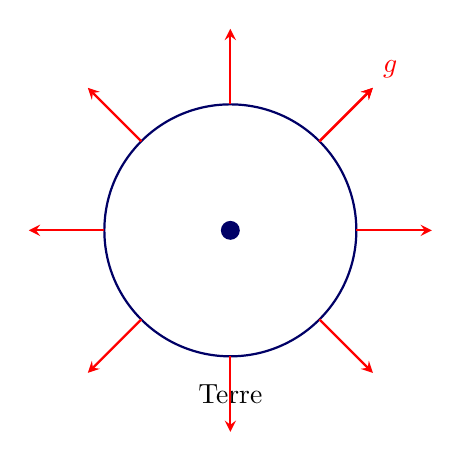
\begin{tikzpicture}[scale=0.8]
\draw[thick,blue!40!black] (0,0) circle (2);
\fill[blue!40!black] (0,0) circle (0.15);
\node[below] at (0,-2.3) {Terre};
\foreach \ang in {0,45,...,315}
{
\draw[->,>=stealth,thick,red] (\ang:2) -- (\ang:3.2);
}
\draw[->,>=stealth,thick,red] (45:2) -- (45:3.2) node[above right] {$\vect{g}$};
\end{tikzpicture}
\fig{Champ de gravitation terrestre : vecteurs $\vect{g}$ radiaux et centripètes.}
\end{illus}

% ===================================================================
\section{Champ électrostatique}

\subsection{Loi de Coulomb}

\begin{loi}[Coulomb]
Deux charges ponctuelles $q_1$ et $q_2$, distantes de $r$, exercent l’une sur l’autre une force :
\[
\vect{F}_{1\to2} = \frac{1}{4\pi\varepsilon_0}\,\frac{q_1 q_2}{r^2}\,\vect{u}_{12}
\]
avec $\varepsilon_0 = \SI{8.85e-12}{\farad\per\metre}$ (permittivité du vide). La force est attractive si $q_1 q_2 < 0$, répulsive si $q_1 q_2 > 0$.
\end{loi}

\subsection{Champ créé par une charge ponctuelle}

\begin{definition}[Champ électrostatique]
Le champ électrostatique créé par une charge $q$ en un point distant de $r$ est :
\[
\vect{E}(r) = \frac{1}{4\pi\varepsilon_0}\,\frac{q}{r^2}\,\vect{u}_r
\]
Unité : $\si{\volt\per\metre}$ (ou $\si{\newton\per\coulomb}$).
\end{definition}

\begin{exemple}
Pour $q = \SI{1e-9}{\coulomb}$ à $r = \SI{10}{\centi\metre}$ :
\[
E = \frac{9\times10^9 \times 10^{-9}}{(0,10)^2} = \SI{900}{\volt\per\metre}
\]
\end{exemple}

\subsection{Superposition de plusieurs charges}

\begin{propriete}[Principe de superposition]
Le champ total en un point est la somme vectorielle des champs créés par chaque charge :
\[
\vect{E}_{\text{tot}} = \sum_i \vect{E}_i
\]
\end{propriete}

\begin{illus}
\begin{tikzpicture}[scale=0.9]
\coordinate (A) at (-2,0);
\coordinate (B) at (2,0);
\coordinate (M) at (0,1.5);
\fill[red] (A) circle (0.08) node[below] {$+q$};
\fill[blue] (B) circle (0.08) node[below] {$-q$};
\draw[->,>=stealth,thick,red] (M) -- ++(-0.8,0.6) node[above] {$\vect{E}_+$};
\draw[->,>=stealth,thick,blue] (M) -- ++(0.8,0.6) node[above] {$\vect{E}_-$};
\draw[->,>=stealth,ultra thick,black!60!green] (M) -- ++(0,1.2) node[right] {$\vect{E}_{\text{tot}}$};
\end{tikzpicture}
\fig{Superposition des champs de deux charges opposées (dipôle).}
\end{illus}

\subsection{Champ dans un condensateur plan}

\begin{definition}[Condensateur plan]
Deux plaques métalliques parallèles, séparées par une distance $d$, portant des charges $+Q$ et $-Q$, créent entre elles un champ électrostatique \textbf{uniforme} :
\[
E = \frac{U}{d} \quad\text{et}\quad \vect{E} \text{ est perpendiculaire aux plaques, dirigé de $+$ vers $-$}
\]
où $U$ est la tension entre les armatures.
\end{definition}

\begin{illus}
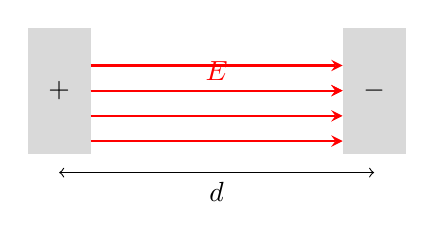
\begin{tikzpicture}[scale=0.8]
\fill[gray!30] (-3,0) rectangle (-2,2);
\fill[gray!30] (2,0) rectangle (3,2);
\node at (-2.5,1) {$+$};
\node at (2.5,1) {$-$};
\foreach \y in {0.2,0.6,...,1.8}
{
\draw[->,>=stealth,thick,red] (-2,\y) -- (2,\y);
}
\draw[->,>=stealth,thick,red] (-2,1) -- (2,1) node[midway,above] {$\vect{E}$};
\draw[<->] (-2.5,-0.3) -- (2.5,-0.3) node[midway,below] {$d$};
\end{tikzpicture}
\fig{Champ uniforme dans un condensateur plan.}
\end{illus}

\begin{aretenir}
Le champ électrostatique est \textbf{uniforme} entre les armatures d’un condensateur plan : même direction, même sens, même intensité en tout point.
\end{aretenir}

% ===================================================================
\section{Champ magnétique}

\subsection{Sources du champ magnétique}

Le champ magnétique $\vect{B}$ (unité : le tesla, $\si{\tesla}$) est créé par :
\begin{itemize}
\item les \textbf{aimants} permanents (pôle nord → pôle sud à l’extérieur) ;
\item les \textbf{courants électriques} (conducteurs parcourus par un courant).
\end{itemize}

\begin{experience}[Spectre magnétique]
Saupoudrer de la limaille de fer autour d’un aimant droit ou en U : les particules s’orientent selon les lignes de champ.
\end{experience}

\imgreal{ch01-spectre-aimant-droit.jpg}{Figure — Spectre magnétique d’un aimant droit obtenu avec de la limaille de fer : lignes allant …}

\subsection{Champ magnétique terrestre}

\begin{propriete}
La Terre se comporte comme un aimant : son champ magnétique $\vect{B}_T$ a une intensité d’environ $\SI{5e-5}{\tesla}$ à l’équateur. Le pôle nord magnétique est proche du pôle sud géographique.
\end{propriete}

\subsection{Champ créé par un courant}

\subsubsection{Fil rectiligne infini}

\begin{loi}[Biot et Savart — fil rectiligne]
Un fil rectiligne infini parcouru par un courant $I$ crée à une distance $r$ un champ magnétique :
\[
B = \frac{\mu_0 I}{2\pi r}
\]
où $\mu_0 = 4\pi\times10^{-7}\,\si{\tesla\metre\per\ampere}$ est la perméabilité du vide.
\end{loi}

\begin{remarque}
Les lignes de champ sont des cercles centrés sur le fil. Le sens est donné par la \textbf{règle de la main droite} : pouce dans le sens du courant, les doigts indiquent le sens de $\vect{B}$.
\end{remarque}

\begin{illus}
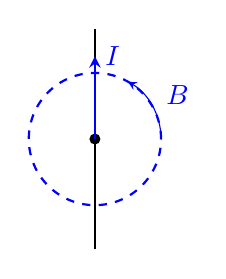
\begin{tikzpicture}[scale=0.7]
\draw[thick] (0,-2) -- (0,2);
\fill[black] (0,0) circle (0.1);
\draw[->,>=stealth,thick,blue] (0,0) -- (0,1.5) node[right] {$I$};
\draw[thick,blue,dashed] (0,0) circle (1.2);
\draw[->,>=stealth,blue] (1.2,0) arc (0:60:1.2);
\node[blue] at (1.5,0.8) {$\vect{B}$};
\end{tikzpicture}
\fig{Lignes de champ circulaires autour d’un fil rectiligne.}
\end{illus}

\subsubsection{Spire circulaire}

Au centre d’une spire de rayon $R$ parcourue par $I$ :
\[
B = \frac{\mu_0 I}{2R}
\]

\subsubsection{Solénoïde}

\begin{definition}[Solénoïde]
Un solénoïde est un enroulement cylindrique de $N$ spires, de longueur $\ell$, parcouru par un courant $I$. À l’intérieur, le champ est \textbf{uniforme} :
\[
B = \mu_0\,\frac{N}{\ell}\,I = \mu_0 n I
\]
où $n = N/\ell$ est la densité linéique de spires.
\end{definition}

\begin{illus}
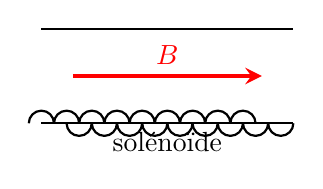
\begin{tikzpicture}[scale=0.8]
\draw[thick] (0,0) -- (4,0);
\draw[thick] (0,1.5) -- (4,1.5);
\foreach \x in {0.2,0.6,...,3.8}
{
\draw[thick] (\x,0) arc (0:180:0.2);
\draw[thick] (\x+0.2,0) arc (180:360:0.2);
}
\draw[->,>=stealth,ultra thick,red] (0.5,0.75) -- (3.5,0.75) node[midway,above] {$\vect{B}$};
\node at (2,-0.3) {solénoïde};
\end{tikzpicture}
\fig{Champ magnétique uniforme à l’intérieur d’un solénoïde.}
\end{illus}

\begin{aretenir}
Le champ magnétique est \textbf{uniforme} à l’intérieur d’un solénoïde long et nul à l’extérieur (en première approximation).
\end{aretenir}

% ===================================================================
\section{Lignes de champ et spectres}

\begin{definition}[Lignes de champ]
Une ligne de champ est une courbe telle qu’en chacun de ses points, le vecteur champ lui est tangent. Le sens de la ligne est celui du vecteur champ.
\end{definition}

\begin{propriete}
\begin{itemize}
\item Les lignes de champ \textbf{ne se coupent pas}.
\item Leur densité est proportionnelle à l’intensité du champ.
\item Pour un champ uniforme, les lignes sont parallèles et équidistantes.
\end{itemize}
\end{propriete}

\imgreal{ch01-spectre-aimant-u.jpg}{Figure — Spectre magnétique d’un aimant en U : lignes quasi parallèles entre les pôles (champ un…}

% ===================================================================
\section{Superposition des champs}

\begin{propriete}[Principe de superposition]
Le champ résultant en un point est la somme vectorielle des champs créés par chaque source :
\[
\vect{g}_{\text{tot}} = \sum \vect{g}_i \qquad \vect{E}_{\text{tot}} = \sum \vect{E}_i \qquad \vect{B}_{\text{tot}} = \sum \vect{B}_i
\]
\end{propriete}

\begin{exemple}
Deux fils parallèles parcourus par des courants de même sens : les champs s’annulent au milieu si les courants sont égaux.
\end{exemple}

% ===================================================================
\section{L’essentiel à retenir}

\begin{synthese}
\begin{itemize}
\item \textbf{Champ de gravitation} : $\vect{g} = -G\frac{M}{r^2}\vect{u}_r$ ; à la surface de la Terre $g = \SI{9.8}{\newton\per\kilogram}$.
\item \textbf{Champ électrostatique} : $\vect{E} = \frac{1}{4\pi\varepsilon_0}\frac{q}{r^2}\vect{u}_r$ ; dans un condensateur plan $E = U/d$.
\item \textbf{Champ magnétique} : fil rectiligne $B = \mu_0 I/(2\pi r)$ ; solénoïde $B = \mu_0 n I$.
\item \textbf{Lignes de champ} : tangentes au vecteur champ, ne se coupent pas.
\item \textbf{Superposition} : le champ total est la somme vectorielle des champs individuels.
\item \textbf{Unités} : $g$ en $\si{\newton\per\kilogram}$ ou $\si{\metre\per\second\squared}$ ; $E$ en $\si{\volt\per\metre}$ ; $B$ en $\si{\tesla}$.
\end{itemize}
\end{synthese}

% ===================================================================
\section{Méthodes \& savoir-faire}

\methode{Calculer un champ de gravitation}
Pour déterminer $\vect{g}$ à une altitude $h$ : $g(h) = G M_T/(R_T + h)^2$. Attention à ne pas confondre $g$ et $G$.

\begin{exemple}
Calculer $g$ à $h = \SI{100}{\kilo\metre}$ ($R_T = \SI{6400}{\kilo\metre}$, $M_T = \SI{6.0e24}{\kilogram}$).
\[
g = \frac{6,67\times10^{-11}\times6,0\times10^{24}}{(6,5\times10^{6})^2} = \SI{9.47}{\newton\per\kilogram}
\]
\end{exemple}

\methode{Calculer un champ électrostatique résultant}
Décomposer chaque charge, calculer $E_i = k|q_i|/r_i^2$, projeter sur les axes, sommer.

\begin{exemple}
Deux charges $q_1 = \SI{2}{\nano\coulomb}$ en $(-a,0)$ et $q_2 = \SI{-2}{\nano\coulomb}$ en $(a,0)$ avec $a = \SI{5}{\centi\metre}$. Champ en $(0,a)$.
\[
E_1 = E_2 = \frac{9\times10^9\times2\times10^{-9}}{(0,05\sqrt{2})^2} = \SI{3.6e3}{\volt\per\metre}
\]
Par symétrie, $\vect{E}_{\text{tot}}$ est vertical descendant : $E_{\text{tot}} = 2E_1\cos45^\circ = \SI{5.09e3}{\volt\per\metre}$.
\end{exemple}

\methode{Utiliser la règle de la main droite}
Pouce = sens du courant ; doigts = sens du champ magnétique (pour un fil rectiligne). Pour une spire, les doigts suivent le courant, le pouce donne le sens du champ au centre.

\methode{Reconnaître un champ uniforme}
Lignes de champ parallèles et équidistantes. Exemples : condensateur plan, intérieur d’un solénoïde long, champ de pesanteur à petite échelle.

\methode{Appliquer le principe de superposition}
Toujours travailler vectoriellement. Utiliser un repère, projeter, additionner les composantes.

% ===================================================================
\section{Exercices d’application}

\rubrique{Champ de gravitation}

\exo{}\diff{1} Calculer l’intensité du champ de gravitation à la surface de la Lune ($M_L = \SI{7.35e22}{\kilogram}$, $R_L = \SI{1.74e6}{\metre}$).

\exo{}\diff{2} À quelle altitude $h$ le champ $g$ vaut-il la moitié de sa valeur au sol ($g_0 = \SI{9.8}{\newton\per\kilogram}$) ? Donnée : $R_T = \SI{6400}{\kilo\metre}$.

\rubrique{Champ électrostatique}

\exo{}\diff{1} Une charge $q = \SI{3}{\nano\coulomb}$ est placée à l’origine. Calculer $\vect{E}$ au point $M(0, \SI{4}{\centi\metre})$.

\exo{}\diff{2} Deux charges $q_1 = \SI{4}{\nano\coulomb}$ et $q_2 = \SI{-4}{\nano\coulomb}$ sont placées en $(-3,0)$ et $(3,0)$ (en cm). Déterminer $\vect{E}$ au point $(0,4)$ cm.

\exo{}\diff{3} Un condensateur plan a des armatures distantes de $d = \SI{2}{\milli\metre}$ et une tension $U = \SI{100}{\volt}$. Calculer $E$ et la force sur un électron ($e = \SI{1.6e-19}{\coulomb}$) placé entre les armatures.

\rubrique{Champ magnétique}

\exo{}\diff{1} Un fil rectiligne parcouru par $I = \SI{5}{\ampere}$. Calculer $B$ à $r = \SI{10}{\centi\metre}$.

\exo{}\diff{2} Un solénoïde de longueur $\ell = \SI{30}{\centi\metre}$ comporte $N = 600$ spires et est parcouru par $I = \SI{2}{\ampere}$. Calculer $B$ à l’intérieur.

\exo{}\diff{3} Deux fils parallèles distants de $d = \SI{20}{\centi\metre}$ sont parcourus par $I_1 = I_2 = \SI{10}{\ampere}$ en sens contraires. Calculer $B$ au milieu des deux fils.

\rubrique{Lignes de champ et superposition}

\exo{}\diff{2} Représenter qualitativement les lignes de champ d’un dipôle électrostatique ($+q$ et $-q$ séparés par une distance $d$).

\exo{}\diff{3} On superpose un champ électrique uniforme $\vect{E}_0 = E_0\,\vect{u}_x$ et le champ d’une charge $+q$ placée à l’origine. Décrire qualitativement les lignes de champ résultantes.

% ===================================================================
\section{Exercices d’entraînement}

\rubrique{Champ de gravitation}

\exo{}\diff{2} La station spatiale internationale orbite à $h = \SI{400}{\kilo\metre}$. Calculer $g$ à cette altitude. Les astronautes sont en apesanteur apparente : pourquoi ?

\exo{}\diff{3} Deux masses $m_1 = \SI{100}{\kilogram}$ et $m_2 = \SI{200}{\kilogram}$ sont distantes de $d = \SI{1}{\metre}$. Où placer une troisième masse $m_3$ pour que la force gravitationnelle totale sur elle soit nulle ?

\exo{}\diff{1} Comparer $g$ à l’équateur et aux pôles (la Terre n’est pas parfaitement sphérique). Donnée : $R_{\text{équateur}} = \SI{6378}{\kilo\metre}$, $R_{\text{pôle}} = \SI{6357}{\kilo\metre}$.

\rubrique{Champ électrostatique}

\exo{}\diff{2} Quatre charges $+q$ sont placées aux sommets d’un carré de côté $a$. Calculer $\vect{E}$ au centre du carré.

\exo{}\diff{3} Un pendule électrostatique (boule de masse $m = \SI{1}{\gram}$, charge $q = \SI{0.5}{\micro\coulomb}$) est placé dans un champ uniforme $\vect{E}$ horizontal. À l’équilibre, le fil fait un angle $\theta = 15^\circ$ avec la verticale. Calculer $E$.

\exo{}\diff{2} Dans un condensateur plan, on injecte un électron avec une vitesse initiale $\vect{v}_0$ parallèle aux armatures. Décrire sa trajectoire.

\rubrique{Champ magnétique}

\exo{}\diff{2} Deux spires coaxiales de rayon $R = \SI{10}{\centi\metre}$, distantes de $R$, sont parcourues par le même courant $I = \SI{2}{\ampere}$ dans le même sens. Calculer $B$ au centre du système (bobines de Helmholtz).

\exo{}\diff{3} Un solénoïde de $N = 1000$ spires, $\ell = \SI{50}{\centi\metre}$, $I = \SI{3}{\ampere}$. On place une aiguille aimantée à l’intérieur. Quel angle fait-elle avec l’axe si on superpose un champ terrestre horizontal $B_T = \SI{2e-5}{\tesla}$ perpendiculaire à l’axe ?

\exo{}\diff{1} Un fil rectiligne et une spire carrée de côté $a$ sont dans le même plan. Le fil est parallèle à un côté de la spire, à distance $d$. Le courant dans le fil est $I_1$, dans la spire $I_2$. Calculer la force magnétique résultante sur la spire.

\rubrique{Superposition et synthèse}

\exo{}\diff{3} On dispose d’un condensateur plan vertical créant un champ $\vect{E}$ horizontal et d’un solénoïde horizontal créant $\vect{B}$ perpendiculaire à $\vect{E}$. Un électron pénètre dans la zone avec $\vect{v}_0$ perpendiculaire aux deux champs. À quelle condition sa trajectoire est-elle rectiligne ?

\exo{}\diff{2} Représenter les lignes de champ d’un aimant droit et d’un aimant en U. Expliquer pourquoi le champ est quasi uniforme dans l’entrefer de l’aimant en U.

% ===================================================================
\section{Sujets type Baccalauréat}

\sujetbac[Champ électrostatique et mouvement de particule]

Un faisceau d’électrons (charge $-e$, masse $m_e$) pénètre avec une vitesse $\vect{v}_0 = v_0\,\vect{u}_x$ entre les armatures d’un condensateur plan de longueur $L = \SI{10}{\centi\metre}$, distance $d = \SI{2}{\centi\metre}$, tension $U = \SI{200}{\volt}$. Le champ $\vect{E}$ est vertical vers le haut.

\begin{enumerate}[label=\arabic*)]
\item Calculer l’intensité $E$ du champ électrostatique.
\item Établir les équations horaires du mouvement de l’électron.
\item Déterminer la déflexion verticale $y$ à la sortie du condensateur.
\item L’électron sort-il du condensateur ? Justifier.
\end{enumerate}

Données : $e = \SI{1.6e-19}{\coulomb}$, $m_e = \SI{9.1e-31}{\kilogram}$, $v_0 = \SI{2e7}{\metre\per\second}$.

\sujetbac[Champ magnétique terrestre et boussole]

On modélise le champ magnétique terrestre par un champ uniforme $\vect{B}_T$ horizontal d’intensité $B_T = \SI{2e-5}{\tesla}$. On place une petite aiguille aimantée au centre d’un solénoïde horizontal d’axe perpendiculaire à $\vect{B}_T$. Le solénoïde a $N = 500$ spires, $\ell = \SI{40}{\centi\metre}$.

\begin{enumerate}[label=\arabic*)]
\item Calculer le champ $\vect{B}_S$ créé par le solénoïde lorsqu’il est parcouru par un courant $I = \SI{1}{\ampere}$.
\item L’aiguille s’oriente suivant le champ résultant. Quel angle fait-elle avec $\vect{B}_T$ ?
\item Pour quel courant $I$ l’aiguille fait-elle un angle de $45^\circ$ avec $\vect{B}_T$ ?
\end{enumerate}

\sujetbac[Gravitation et satellites]

Un satellite météorologique de masse $m = \SI{500}{\kilogram}$ est placé sur une orbite circulaire à l’altitude $h = \SI{800}{\kilo\metre}$.

\begin{enumerate}[label=\arabic*)]
\item Calculer l’intensité du champ de gravitation $g(h)$ à cette altitude.
\item En déduire la vitesse $v$ du satellite sur son orbite.
\item Déterminer sa période de révolution $T$.
\item Le satellite est-il géostationnaire ? Justifier.
\end{enumerate}

Données : $R_T = \SI{6400}{\kilo\metre}$, $M_T = \SI{6.0e24}{\kilogram}$, $G = \SI{6.67e-11}{\newton\metre\squared\per\kilogram\squared}$.

% ===================================================================
\section{Corrigés}

\corrige{de l’exercice 1 (Champ de gravitation)}
\[
g_L = G\frac{M_L}{R_L^2} = \frac{6,67\times10^{-11}\times7,35\times10^{22}}{(1,74\times10^{6})^2} = \SI{1.62}{\newton\per\kilogram}
\]

\corrige{de l’exercice 2 (Champ de gravitation)}
\[
\frac{g_0}{2} = \frac{GM_T}{(R_T+h)^2} \Rightarrow (R_T+h)^2 = 2R_T^2 \Rightarrow h = R_T(\sqrt{2}-1) = \SI{2650}{\kilo\metre}
\]

\corrige{de l’exercice 1 (Champ électrostatique)}
\[
E = \frac{1}{4\pi\varepsilon_0}\frac{q}{r^2} = \frac{9\times10^9\times3\times10^{-9}}{(0,04)^2} = \SI{1.69e4}{\volt\per\metre}
\]
Direction : verticale vers le haut (charge positive).

\corrige{de l’exercice 2 (Champ électrostatique)}
$r = \SI{5}{\centi\metre}$, $E_1 = E_2 = \frac{9\times10^9\times4\times10^{-9}}{(0,05)^2} = \SI{1.44e4}{\volt\per\metre}$.
Par symétrie, $\vect{E}_{\text{tot}}$ est vertical descendant :
\[
E_{\text{tot}} = 2E_1\cos\theta \quad\text{avec }\cos\theta = \frac{4}{5} \Rightarrow E_{\text{tot}} = \SI{2.30e4}{\volt\per\metre}
\]

\corrige{de l’exercice 3 (Champ électrostatique)}
\[
E = \frac{U}{d} = \frac{100}{2\times10^{-3}} = \SI{5e4}{\volt\per\metre}
\]
Force sur l’électron : $F = eE = 1,6\times10^{-19}\times5\times10^{4} = \SI{8e-15}{\newton}$.

\corrige{de l’exercice 1 (Champ magnétique)}
\[
B = \frac{\mu_0 I}{2\pi r} = \frac{4\pi\times10^{-7}\times5}{2\pi\times0,10} = \SI{1e-5}{\tesla}
\]

\corrige{de l’exercice 2 (Champ magnétique)}
\[
n = \frac{N}{\ell} = \frac{600}{0,30} = \num{2000}~\mathrm{spires/m} \quad\Rightarrow\quad B = \mu_0 n I = 4\pi\times10^{-7}\times2000\times2 = \SI{5.03e-3}{\tesla}
\]

\corrige{de l’exercice 3 (Champ magnétique)}
Au milieu, les champs des deux fils sont dans le même sens (règle de la main droite) :
\[
B_1 = B_2 = \frac{\mu_0 I}{2\pi(d/2)} = \frac{4\pi\times10^{-7}\times10}{2\pi\times0,10} = \SI{2e-5}{\tesla}
\]
\[
B_{\text{tot}} = B_1 + B_2 = \SI{4e-5}{\tesla}
\]

\corrige{de l’exercice 1 (Lignes de champ et superposition)}
Les lignes de champ partent de la charge $+q$ et aboutissent sur la charge $-q$. Elles sont courbes, plus denses près des charges.

\corrige{de l’exercice 2 (Lignes de champ et superposition)}
Les lignes de champ sont déformées par le champ uniforme : elles partent de la charge et se referment à l’infini en s’alignant avec $\vect{E}_0$.

\corrige{du sujet 1 (Champ électrostatique et mouvement de particule)}
\begin{enumerate}[label=\arabic*)]
\item $E = U/d = 200/(2\times10^{-2}) = \SI{1e4}{\volt\per\metre}$.
\item $\vect{a} = -\frac{e}{m_e}E\,\vect{u}_y$ ; $x = v_0 t$, $y = -\frac{1}{2}\frac{eE}{m_e}t^2$.
\item Temps de traversée : $t = L/v_0 = 0,10/(2\times10^7) = \SI{5e-9}{\second}$.
\[
y = -\frac{1}{2}\frac{1,6\times10^{-19}\times10^4}{9,1\times10^{-31}}\times(5\times10^{-9})^2 = -\SI{2.2e-2}{\metre} = -\SI{2.2}{\centi\metre}
\]
\item $|y| = \SI{2.2}{\centi\metre} > d/2 = \SI{1}{\centi\metre}$ : l’électron sort du condensateur (il heurte l’armature supérieure).
\end{enumerate}

\corrige{du sujet 2 (Champ magnétique terrestre et boussole)}
\begin{enumerate}[label=\arabic*)]
\item $B_S = \mu_0 n I = 4\pi\times10^{-7}\times(500/0,40)\times1 = \SI{1.57e-3}{\tesla}$.
\item $\tan\theta = B_S/B_T = 1,57\times10^{-3}/(2\times10^{-5}) = 78,5 \Rightarrow \theta \approx 89,3^\circ$.
\item $\tan45^\circ = 1 = B_S/B_T \Rightarrow B_S = B_T \Rightarrow I = \frac{B_T}{\mu_0 n} = \frac{2\times10^{-5}}{4\pi\times10^{-7}\times1250} \approx \SI{1.27e-2}{\ampere}$.
\end{enumerate}

\corrige{du sujet 3 (Gravitation et satellites)}
\begin{enumerate}[label=\arabic*)]
\item $g(h) = \frac{GM_T}{(R_T+h)^2} = \frac{6,67\times10^{-11}\times6,0\times10^{24}}{(7,2\times10^{6})^2} = \SI{7.72}{\newton\per\kilogram}$.
\item $v = \sqrt{g(h)(R_T+h)} = \sqrt{7,72\times7,2\times10^{6}} = \SI{7.46e3}{\metre\per\second}$.
\item $T = \frac{2\pi(R_T+h)}{v} = \frac{2\pi\times7,2\times10^{6}}{7,46\times10^{3}} = \SI{6060}{\second} \approx \SI{1.68}{\hour}$.
\item Non, un satellite géostationnaire doit avoir $T = \SI{24}{\hour}$ et être dans le plan équatorial.
\end{enumerate}

\endinput